%=============================================================================
%  LunarLeaf-CFD -- draft manuscript, npj Microgravity style
%  Self-contained: compiles with a standard TeX distribution (pdflatex).
%    pdflatex manuscript.tex ; pdflatex manuscript.tex   (two passes for refs)
%  Figures are read from ../figures/ (PNG). Tables are typeset inline.
%  To submit to a Springer Nature journal, the body can be dropped into the
%  official sn-jnl.cls template with minimal change.
%=============================================================================
\documentclass[10pt]{article}

\usepackage[utf8]{inputenc}
\usepackage[T1]{fontenc}
\usepackage[a4paper,margin=2.3cm]{geometry}
\usepackage{graphicx}
\usepackage{amsmath,amssymb}
\usepackage[super,sort&compress]{natbib}
\usepackage{authblk}
\usepackage{booktabs}
\usepackage{caption}
\usepackage{xcolor}
\usepackage[colorlinks=true,linkcolor=blue!55!black,citecolor=blue!55!black,urlcolor=blue!55!black]{hyperref}
\usepackage{microtype}
% plain-text unit helpers (no siunitx dependency; math-safe via \ensuremath)
\newcommand{\ums}{\ensuremath{\mu\mathrm{mol\,m^{-2}\,s^{-1}}}}
\newcommand{\umh}{\ensuremath{\mu\mathrm{mol\,h^{-1}\,cm^{-2}}}}
\newcommand{\cmsu}{\ensuremath{\mathrm{cm\,s^{-1}}}}
\newcommand{\mseu}{\ensuremath{\mathrm{m^{2}\,s^{-1}}}}
\newcommand{\molms}{\ensuremath{\mathrm{mol\,m^{-2}\,s^{-1}}}}
\newcommand{\msq}{\ensuremath{\mathrm{m\,s^{-2}}}}

\captionsetup{labelfont=bf,font=small,labelsep=period}
\renewcommand\Affilfont{\itshape\small}
\setlength{\parskip}{2pt}
\graphicspath{{../figures/}}

% convenience macros
\newcommand{\co}{CO\textsubscript{2}}
\newcommand{\oo}{O\textsubscript{2}}
\newcommand{\wo}{H\textsubscript{2}O}
\newcommand{\umolm}{\ums}

\title{\bfseries Gravity, geometry and enclosure control the gas-exchange boundary layer of \textit{Arabidopsis}: a validated in-browser CFD model linking spaceflight hardware to carbon gain}

\author[1]{Richard J. Barker\thanks{Correspondence: \texttt{admin@cosecloud.com}}}
\author[1]{\textnormal{and collaborators (author list provisional)}}
\affil[1]{MadWest~/~AstroBotany International Research Initiative (AIRI). Affiliations to be finalised.}
\date{}

\begin{document}
\maketitle

\begin{abstract}
\noindent
Plants grown in spaceflight display stress phenotypes whose mechanistic basis remains debated. A long-suspected
contributor is the loss of buoyancy-driven convection in microgravity, which should thicken the unstirred boundary
layer around plant organs and steepen the \oo/\co/\wo{} gradients that govern gas exchange. We test this with a
browser-based lattice-Boltzmann model that solves incompressible flow, multi-species advection--diffusion and
Boussinesq buoyancy under an adjustable gravity vector, validated against four numerical benchmarks and anchored to
measured \textit{Arabidopsis thaliana} whole-plant-chamber gas exchange (net assimilation 3.85\,\ums \co).
Reducing gravity from 1\,\emph{g} to microgravity removes convective ventilation (peak flow $\propto\sqrt{g}\to0$)
and steepens surface gas gaps 1.5--1.8$\times$ at every scale; denser architectures (rosette, microgreen canopy) trap
air and amplify the effect. The forced airflow needed to restore Earth-equivalent boundary layers scales steeply with
planting density ($\approx$~2.6~/~11~/~21~\cmsu for a leaf~/~rosette~/~canopy). Mapping the three ISS
growth systems onto dish boundary conditions, a sealed BRIC dish both drifts toward hypoxia and, once photosynthesis is
made \co-limited, fixes only $\approx$\,1\,\% of the Earth carbon over a 12\,h photoperiod; a micropore-taped
CARA dish sustains $\approx$\,90\,\% and a ventilated VEGGIE system $\approx$\,100\,\%. The model provides a mechanistic
bridge from cabin-scale transport to plant carbon gain and a quantitative design tool for growth hardware.
\end{abstract}

%------------------------------------------------------------------ Introduction
\section{Introduction}
On Earth a photosynthesising leaf warms and humidifies the thin layer of air at its surface. That air becomes buoyant
and rises---a free-convection plume that continuously sweeps the leaf boundary layer, replenishing \co{} and carrying
away \oo{} and water vapour. This buoyancy-driven ventilation sets the boundary-layer conductance that, in series with
stomatal and mesophyll conductances, limits gas exchange.

In microgravity there is no buoyancy: density differences no longer drive motion, so in still air the only transport is
molecular diffusion. The unstirred boundary layer is expected to thicken and the surface-to-bulk gradients of \co{},
\oo{} and water vapour to steepen. This has long been proposed as a mechanism contributing to the altered morphology,
gas exchange and stress signatures of spaceflight-grown plants\citep{kitaya2003,porterfield2002}, and it is
the stated rationale for the forced-ventilation design of modern growth hardware. Yet the effect resists direct
measurement---no whole-chamber sensor resolves the sub-millimetre boundary layer---so a physically grounded model is
valuable for interpreting results and designing hardware.

We build such a model and make it broadly usable: it runs entirely in a web browser. We (i)~validate an incompressible
flow~+~multi-species transport solver with a user-controlled gravity vector; (ii)~anchor it to measured
\textit{Arabidopsis} gas-exchange rates; (iii)~quantify how reduced gravity reshapes the boundary layer across a single
leaf, a rosette and a dense microgreen canopy; (iv)~compute the forced airflow that counteracts the microgravity
penalty at each scale; (v)~map the three ISS growth systems (BRIC, CARA, VEGGIE) onto solver boundary conditions; and
(vi)~close the loop with \co-limited photosynthesis, translating transport limitation into carbon gain. Throughout we
separate what the data \emph{validate} (flux magnitude, closed-chamber transport) from what the model \emph{predicts}
(the spatial, gravity- and scale-dependent gradients).

%------------------------------------------------------------------ Results
\section{Results}

\subsection{Solver validation}
The solver reproduces four independent benchmarks (Table~\ref{tab:gates}): the Ghia \textit{et al.}\citep{ghia1982}
lid-driven-cavity profiles (Re~100, $L_2=0.011$), Kármán shedding of a confined cylinder ($\mathrm{St}=0.192$), the
de Vahl Davis\citep{devahldavis1983} natural-convection Nusselt number (Ra~$10^4$, $\mathrm{Nu}=2.242$ vs $2.238$;
0.18\,\% error) and the analytic error-function diffusion profile ($L_2\approx0$). Gate~3 is decisive: matching the
natural-convection benchmark to 0.18\,\% confirms the buoyancy/gravity coupling, so setting $g=0$ genuinely collapses
convection to the diffusion limit of gate~4.

\begin{table}[t]\centering\small
\caption{Numerical validation gates.}\label{tab:gates}
\begin{tabular}{clll c}
\toprule
Gate & Benchmark & Reference & Model & \\
\midrule
1 & Lid-driven cavity, Re 100 & Ghia \textit{et al.}\ (1982)\citep{ghia1982} & $L_2=0.011$ & \checkmark\\
2 & Cylinder wake, Re 100 & St $\approx$ 0.16 (unconfined) & St $=0.192$ (confined) & \checkmark\\
3 & Natural convection, Ra $10^4$ & de Vahl Davis (1983)\citep{devahldavis1983}, Nu $=2.238$ & Nu $=2.242$ & \checkmark\\
4 & Pure diffusion & $\tfrac12\,\mathrm{erfc}$ analytic & $L_2\approx0$ & \checkmark\\
\bottomrule
\end{tabular}
\end{table}

\subsection{Measured gas exchange anchors the model}
Two independent measurements fix the physical flux (Fig.~\ref{fig:vernier}, Table~\ref{tab:meas}). A whole-plant-chamber
dataset\citep{chew2017} gives net \co{} assimilation 1.38\,\umh
($=3.85\,\ums$) for Col wild-type, respiration
1.18\,\ums ($R/A=0.31$). An independent 4.8\,d Vernier chamber trace
(Fig.~\ref{fig:vernier}) shows diel \oo{} cycling (6.6--32.8\,\%) and humidity swings. These fix the surface
source/sink in physical units.

\begin{figure}[t]\centering
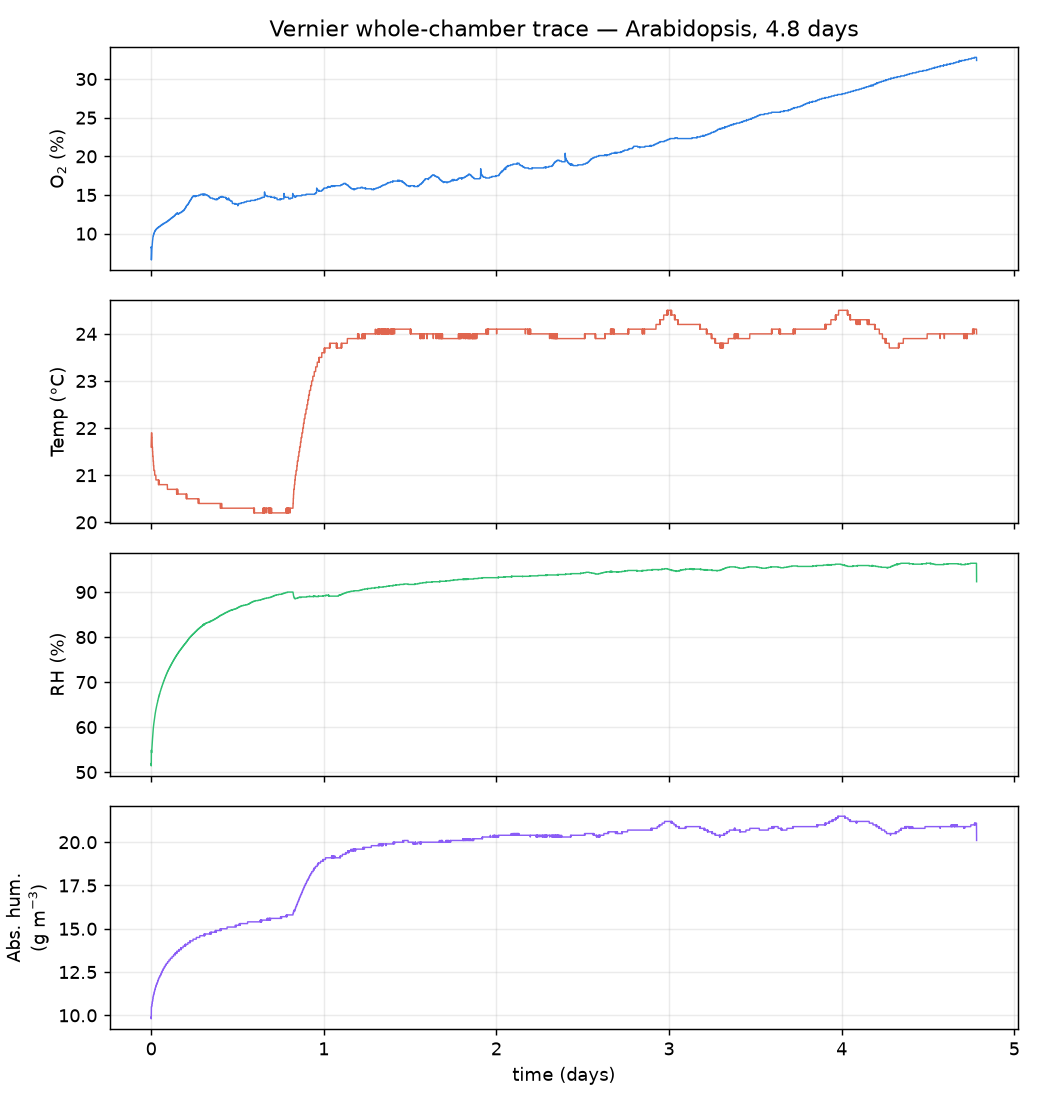
\includegraphics[width=0.62\linewidth]{F1_vernier_timeseries.png}
\caption{\textbf{Measured whole-chamber gas exchange.} Vernier closed-chamber trace over 4.8\,d: \oo,
temperature, relative and absolute humidity, showing plant-driven diel gas cycling.}
\label{fig:vernier}
\end{figure}

\begin{table}[t]\centering\small
\caption{Measured gas exchange (selected).}\label{tab:meas}
\begin{tabular}{lccl}
\toprule
Quantity & Value & Units & Source\\
\midrule
Net \co{} assimilation $A$ & 1.38 (3.85) & \umh (\umolm) & Chamber\citep{chew2017}\\
Dark respiration $R$ & 0.43 (1.18) & \umh (\umolm) & Chamber\citep{chew2017}\\
Chamber volume / area & 339 / 26 & cm\textsuperscript{3} / cm\textsuperscript{2} & Chamber\citep{chew2017}\\
Vernier \oo{} diel range & 6.6--32.8 & \% & Vernier\\
\bottomrule
\end{tabular}
\end{table}

\subsection{Calibration and closed-chamber transport}
Resolving the leaf at 52 cells across a 1.5\,cm blade maps the lattice to $dx=0.288$\,mm,
$dt=0.173$\,ms, an Earth convective velocity $\approx7.7\,\cmsu$ near the leaf. As a sealed chamber
the solver reproduces monotonic accumulation and conserves mass to $2\times10^{-5}$ (Fig.~\ref{fig:chamber}a); a
persistent near-leaf vs far-wall gap develops (Fig.~\ref{fig:chamber}b)---the boundary layer at chamber scale.

\begin{figure}[t]\centering
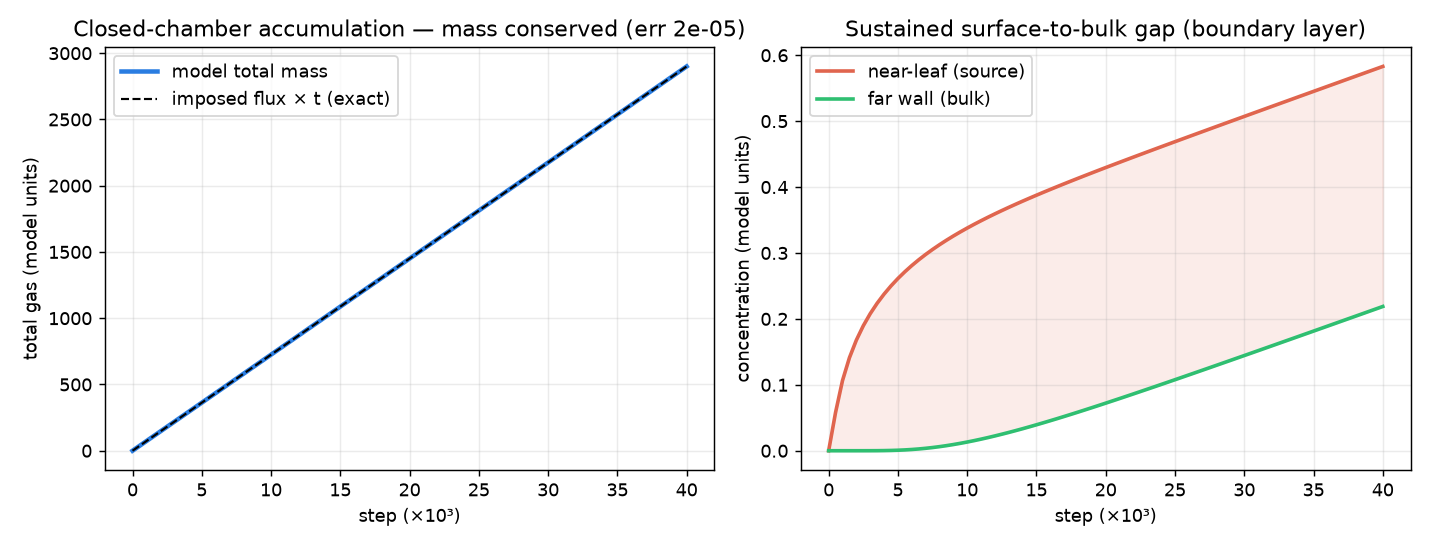
\includegraphics[width=\linewidth]{F5_chamber_validation.png}
\caption{\textbf{Closed-chamber transport validation.} (a)~Sealed-chamber total gas matches the imposed flux (mass
conserved to $2\times10^{-5}$). (b)~Sustained near-leaf vs far-wall gap---the boundary layer at chamber scale.}
\label{fig:chamber}
\end{figure}

\subsection{Gravity controls the boundary layer}
Sweeping gravity from Earth through Mars (0.38\,\emph{g}) and the Moon (0.17\,\emph{g}) to microgravity,
convection weakens ($\propto\sqrt{g}$) while surface gaps steepen (Fig.~\ref{fig:gravscale}a). The field maps
(Fig.~\ref{fig:plume}) show a buoyant plume rising off the leaf at 1\,\emph{g} and a symmetric, thicker diffusive
halo in microgravity; the surface \co{} gap roughly doubles.

\begin{figure}[t]\centering
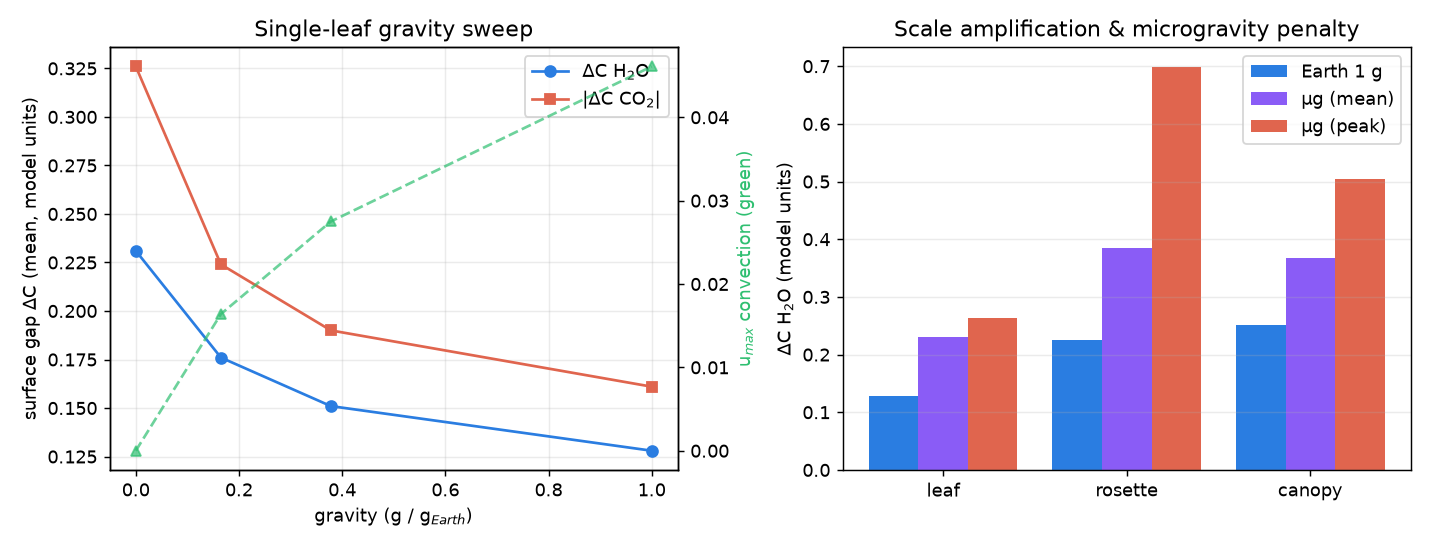
\includegraphics[width=\linewidth]{F4_gravity_scale.png}
\caption{\textbf{Gravity and scale.} (a)~Single-leaf gravity sweep. (b)~Scale amplification and microgravity penalty
across leaf, rosette and canopy.}
\label{fig:gravscale}
\end{figure}

\begin{figure}[t]\centering
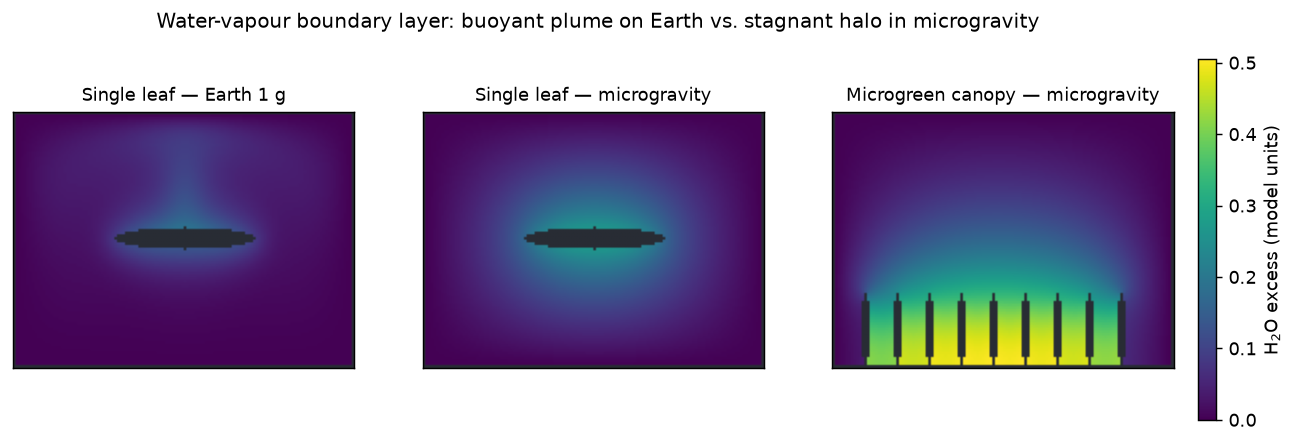
\includegraphics[width=\linewidth]{F3_plume_maps.png}
\caption{\textbf{Water-vapour boundary layer.} Buoyant plume (leaf, Earth), symmetric stagnant halo (leaf,
microgravity) and trapped within-canopy air (canopy, microgravity).}
\label{fig:plume}
\end{figure}

\subsection{Scale amplifies the effect}
From leaf to rosette to canopy the penalty compounds (Fig.~\ref{fig:gravscale}b). Overlapping rosette leaves trap air
in the crown (steepest \emph{local} gradients); the canopy ventilates only at its top and stagnates as a whole (highest
\emph{mean} gradient). Both intensify in microgravity.

\subsection{Physical prediction of surface drawdown}
Anchoring the dimensionless gradients on the measured flux and a still-air leaf boundary-layer conductance
(1.0\,\molms) yields a \co{} drawdown of $\approx$\,4\,ppm (isolated leaf, Earth)
rising to $\approx$\,13\,ppm (rosette bulk, microgravity), with crown pockets $\approx$\,25\,ppm
(Table~\ref{tab:ppm}); these add to stomatal/mesophyll drops.

\begin{table}[t]\centering\small
\caption{Predicted leaf-surface \co{} drawdown (ppm), anchored on the measured flux.}\label{tab:ppm}
\begin{tabular}{lcc}
\toprule
Scenario & Mean & Peak\\
\midrule
Leaf $\cdot$ Earth & 3.8 & 5.9\\
Leaf $\cdot$ microgravity & 7.8 & 8.9\\
Rosette $\cdot$ Earth & 7.1 & 17.1\\
Rosette $\cdot$ microgravity & 13.2 & 24.7\\
Canopy $\cdot$ Earth & 7.8 & 12.9\\
Canopy $\cdot$ microgravity & 10.6 & 14.4\\
\bottomrule
\end{tabular}
\end{table}

\subsection{Forced ventilation reverses the penalty---but the requirement scales with density}
Forced airflow substitutes for the missing buoyant convection. For an isolated leaf, $\approx2.6\,\cmsu$
restores Earth-equivalent gradients (Fig.~\ref{fig:fan}). Across scales the Earth-equivalent airflow rises steeply with
density---$\approx$~2.6, 11 and 21\,\cmsu for leaf, rosette and canopy (Fig.~\ref{fig:fanscale}), an
$\sim8\times$ increase. The canopy is hardest to ventilate: side airflow skims the stand while within-canopy air stays
stagnant, so its curve flattens and only approaches the Earth level near the low-Mach limit.

\begin{figure}[t]\centering
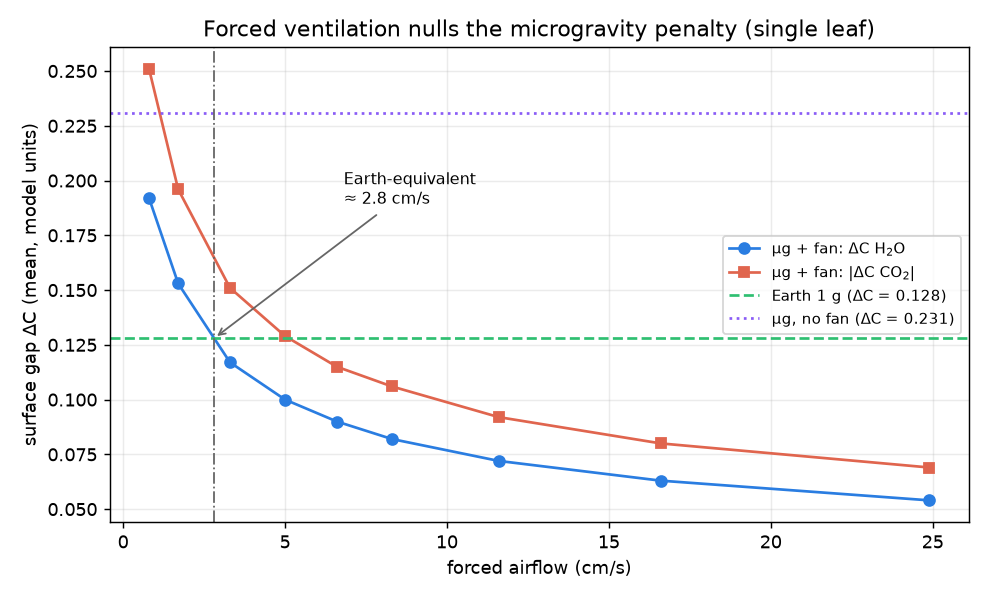
\includegraphics[width=0.72\linewidth]{F6_forced_airflow.png}
\caption{\textbf{Forced ventilation nulls the microgravity penalty (single leaf).} Surface gap vs fan speed, with
Earth-1\,\emph{g} and $\mu$g references and the $\approx2.6\,\cmsu$ Earth-equivalent point.}
\label{fig:fan}
\end{figure}

\begin{figure}[t]\centering
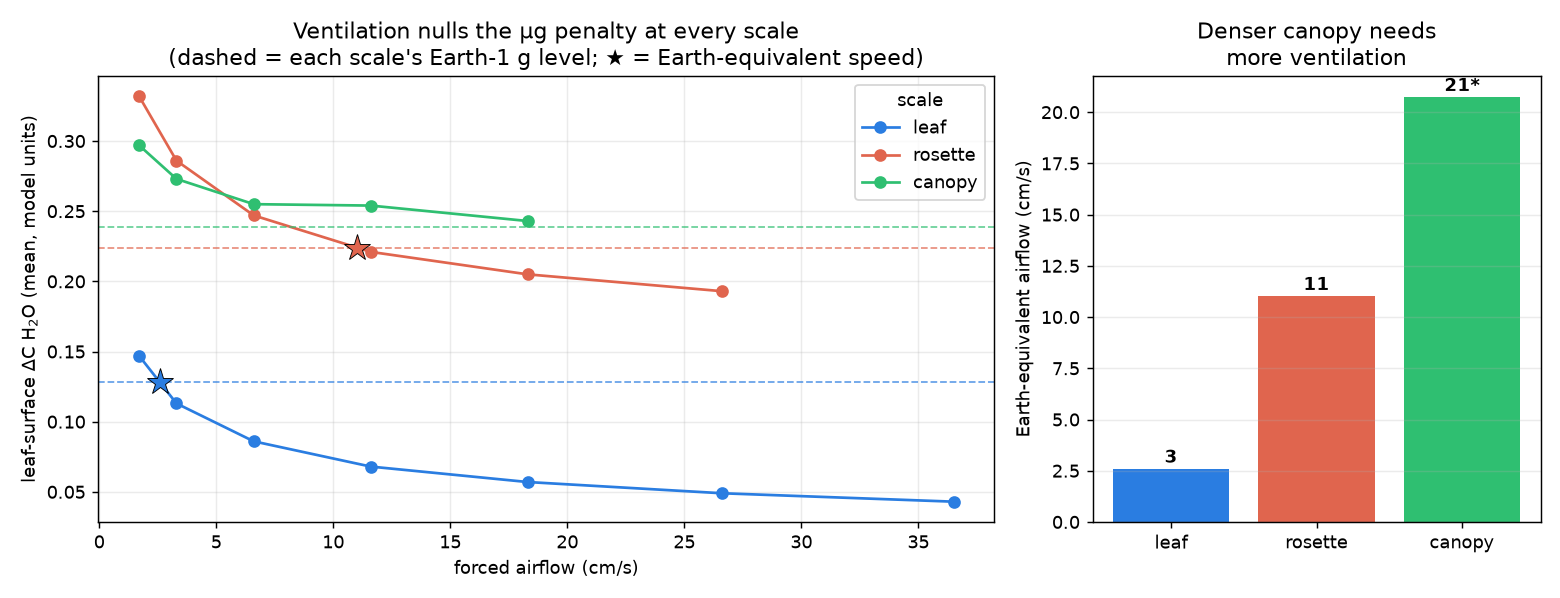
\includegraphics[width=\linewidth]{F8_fan_by_scale.png}
\caption{\textbf{Ventilation requirement scales with planting density.} (a)~Fan-sweep curves per scale with Earth
references and crossings. (b)~Earth-equivalent airflow $\approx$ 2.6~/~11~/~21~\cmsu (canopy extrapolated;
higher speeds exceeded the low-Mach limit).}
\label{fig:fanscale}
\end{figure}

\subsection{Spaceflight hardware as boundary conditions}
The three ISS systems differ, in gas-transport terms, only in the boundary condition on the dish (Figs.~\ref{fig:hw},
\ref{fig:hwscale}). \textbf{BRIC}---hermetically sealed\citep{correll2013}---imposes zero-flux walls: the enclosure
atmosphere drifts without bound (Fig.~\ref{fig:hw}a), and a mass balance (Table~\ref{tab:times}) shows the
$\sim$400\,ppm \co{} in a 30\,cm\textsuperscript{3} headspace is fixed in $\approx$7\,min (light), while in the dark
\co{} reaches 1\,\% in $\approx$9\,h and \oo{} falls to a hypoxic 5\,\% in $\approx$6.5\,d. \textbf{CARA}
---gas-permeable micropore tape\citep{sealingfilm}---vents the dish near ambient (consistent with ground data that
surgical tape holds near-ambient \co/\oo{} while parafilm depletes \co{} and triggers stress genes\citep{sealingfilm,parafilm})
but does not fix the microgravity boundary layer (Fig.~\ref{fig:hwscale}). \textbf{VEGGIE}---light + forced airflow---
vents the enclosure \emph{and} thins the boundary layer ($\sim3\times$ smaller surface gradient). Across all scales
BRIC~$\approx$~CARA at the surface, and one VEGGIE fan speed ($\sim8\,\cmsu$) that restores a leaf barely
helps a rosette or canopy (Fig.~\ref{fig:hwscale}), being below their 11 and 21\,\cmsu needs.

\begin{figure}[t]\centering
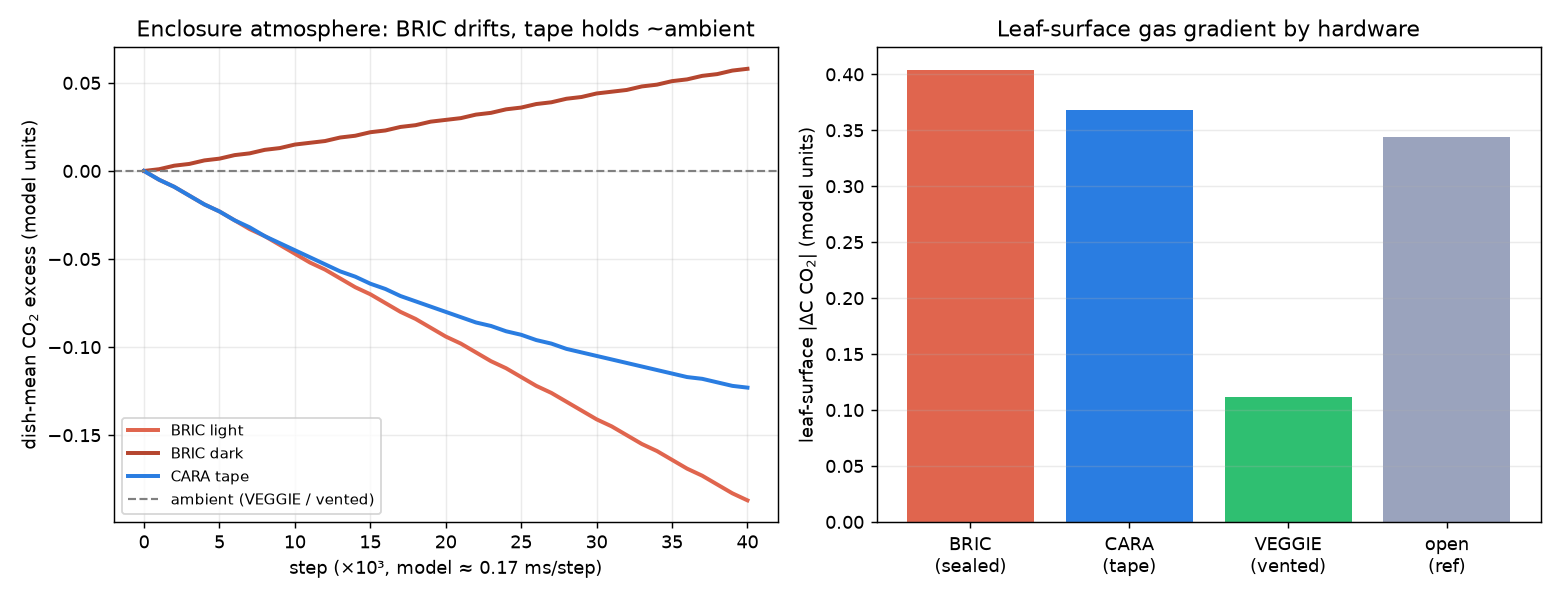
\includegraphics[width=\linewidth]{F7_hardware_compare.png}
\caption{\textbf{Spaceflight hardware as dish boundary conditions.} (a)~Enclosure-mean \co{} drift---BRIC diverges,
the taped dish holds near ambient. (b)~Leaf-surface gradient by hardware.}
\label{fig:hw}
\end{figure}

\begin{figure}[t]\centering
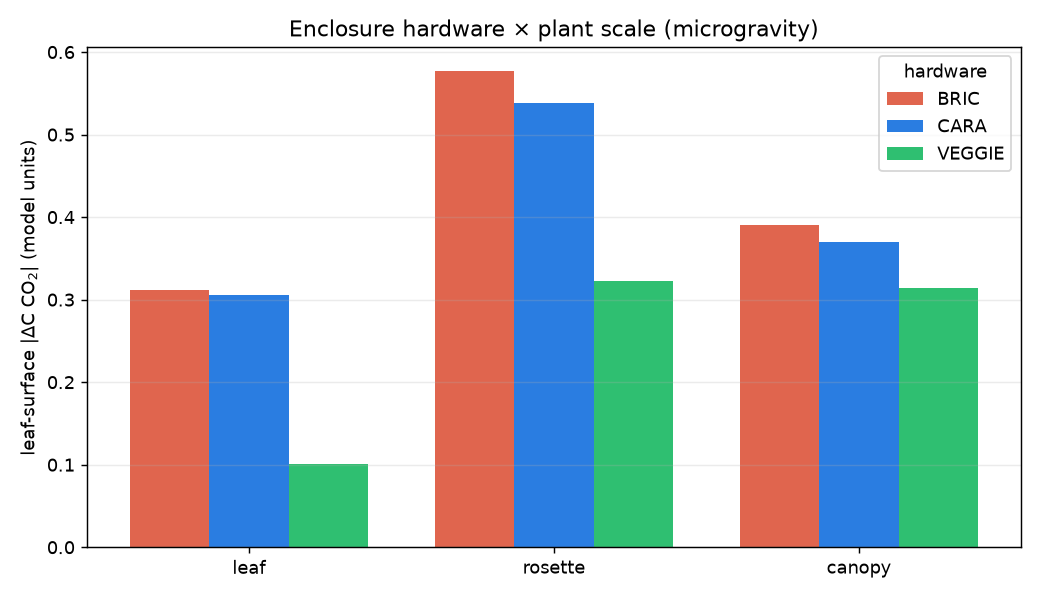
\includegraphics[width=0.78\linewidth]{F9_hardware_by_scale.png}
\caption{\textbf{Hardware $\times$ plant scale (microgravity).} BRIC~$\approx$~CARA at the leaf surface at every scale;
one VEGGIE fan speed under-serves denser stands.}
\label{fig:hwscale}
\end{figure}

\begin{table}[t]\centering\small
\caption{Sealed-dish (BRIC) atmosphere timescales (analytic; 30\,cm\textsuperscript{3} dish, 3\,cm\textsuperscript{2} leaf).}
\label{tab:times}
\begin{tabular}{lc}
\toprule
Event & Time\\
\midrule
Light: \co{} 400\,ppm $\to$ $\sim$0 (photosynthesis self-limits) & $\approx$ 7\,min\\
Dark: \co{} $\to$ 1\,\% (stress) & $\approx$ 9\,h\\
Dark: \oo{} 21 $\to$ 5\,\% (hypoxia) & $\approx$ 6.5\,d\\
\bottomrule
\end{tabular}
\end{table}

\subsection{Closing the loop: \texorpdfstring{\co}{CO2}-limited photosynthesis}
Making \co{} uptake follow a compensation-point + saturation response of the \emph{local} surface \co{}, boundary-layer
depletion self-limits assimilation by $\approx$1--4\,\% at steady state, tracking transport: smallest under ventilation
(VEGGIE, net $A=99.3\,\%$ of potential), larger for a bare microgravity leaf (98.0\,\%) and largest in the trapped
rosette crown (96.5\,\%; Table~\ref{tab:feedback}). Over a 12\,h photoperiod
(Fig.~\ref{fig:feedback}), the sealed BRIC dish's surface \co{} falls to the compensation point within minutes,
photosynthesis collapses, and only $\approx$1\,\% of the Earth carbon is fixed; CARA sustains $\approx$90\,\% and VEGGIE
$\approx$100\,\%. Transport limitations therefore throttle carbon gain---mildly where air moves, almost completely where
it is sealed and still.

\begin{figure}[t]\centering
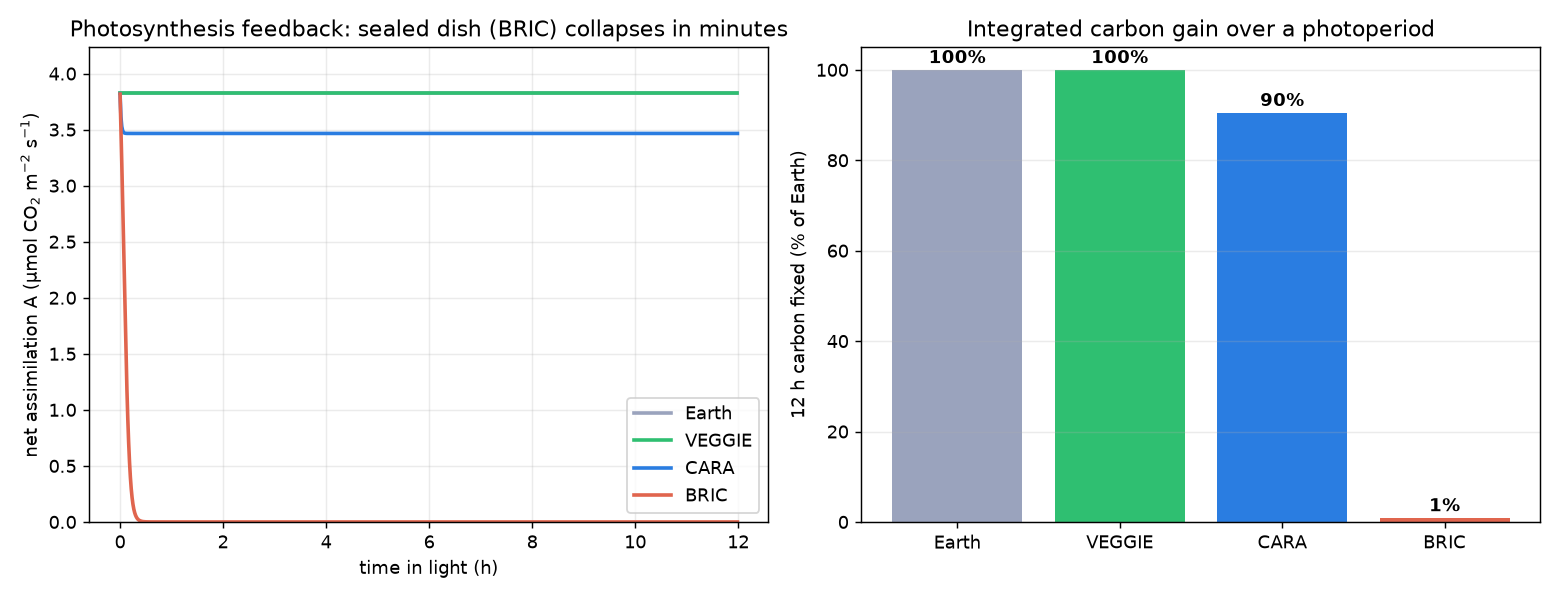
\includegraphics[width=\linewidth]{F10_photosynthesis_feedback.png}
\caption{\textbf{Closed-loop \co-limited photosynthesis.} (a)~Net assimilation over a photoperiod---the sealed BRIC
dish collapses within minutes. (b)~Integrated 12\,h carbon: BRIC $\approx$1\,\%, CARA $\approx$90\,\%, VEGGIE
$\approx$100\,\% of Earth.}
\label{fig:feedback}
\end{figure}

\begin{table}[t]\centering\small
\caption{Closed-loop net assimilation (solver, \% of light-saturated potential).}\label{tab:feedback}
\begin{tabular}{lc}
\toprule
Scenario & Net $A$ (\%)\\
\midrule
Leaf $\cdot$ Earth & 98.9\\
Leaf $\cdot$ microgravity & 98.0\\
Rosette $\cdot$ microgravity (crown) & 96.5\\
Canopy $\cdot$ microgravity & 97.5\\
Leaf $\cdot$ $\mu$g $\cdot$ VEGGIE & 99.3\\
\bottomrule
\end{tabular}
\end{table}

%------------------------------------------------------------------ Discussion
\section{Discussion}
The results give a mechanistic, quantitative account of a long-suspected spaceflight stress: without buoyancy-driven
convection, plant organs sit in a thickened, poorly-ventilated boundary layer that is simultaneously \co-starved,
\oo-enriched and humid. This is not a fixed penalty but one that scales with gravity, canopy architecture and---through
the \co{} feedback---the gas-exchange control of the enclosure. Because the effect is transport- rather than
biochemistry-limited it is engineerable, and the same solver that quantifies it sizes the airflow needed to remove it.
The scale dependence of that requirement ($\approx$2.6~$\to$~11~$\to$~21\,\cmsu) is a concrete design
guideline: a setting tuned on sparse plants under-serves a dense stand. Framing the three ISS systems as a ladder of
gas-exchange control---sealed, vented seal, actively ventilated---and adding the photosynthesis feedback converts these
into a growth currency: a sealed dish fixes almost no carbon over a photoperiod. This offers a parsimonious, physics-based
contributor to the reduced growth and stress transcriptomes of sealed-hardware spaceflight
experiments\citep{correll2013,parafilm}, complementary to gravisensing- and light-driven responses\citep{cara}.
Consistent with a transport-limited mechanism, whole-stand gas exchange in microgravity is unchanged at
saturating \co\citep{monje2005}---exactly the regime in which the boundary-layer \co{} limitation is relieved.

\paragraph{Limitations.} The model is 2-D and Boussinesq (kept within validity, $u_{\max}<0.1$, $\beta\,\Delta C\lesssim0.5$).
Photosynthesis is \co-limited but stomatal \emph{conductance} is not yet dynamic; the \co-response and tape-permeance
parameters are reasonable assumptions, not fits. Absolute $\Delta C$ are lattice units converted to ppm through one
literature-anchored conductance, and the microgravity boundary layer is bounded by the finite chamber, so the reported
gravity ratios are conservative lower bounds. The ground data validate the flux magnitude and closed-chamber transport,
not the spatial boundary layer; the gravity- and scale-dependent gradients remain model predictions on validated
components.

\paragraph{Future work.} Dynamic stomatal conductance; a 3-D WebGPU solver to remove chamber conservatism and allow
turbulent canopy flow; calibration against spatially-resolved surface-gas imaging; and coupling to a whole-plant
carbon-balance model to predict growth across mission durations.

%------------------------------------------------------------------ Methods
\section{Methods}
\paragraph{Flow solver.} Two-dimensional D2Q9 BGK lattice-Boltzmann with halfway bounce-back walls;
$\nu=c_s^2(\tau-\tfrac12)$, $c_s^2=\tfrac13$; body forces via the Guo scheme.
\paragraph{Species transport.} Three species (\co, \oo, \wo) on D2Q5 advection--diffusion lattices sharing the flow,
diffusivity ratio $1.6:2.0:2.4\;(\times10^{-5}\,\mseu)$; walls zero-flux, Dirichlet
(anti-bounce-back) or semi-permeable membrane.
\paragraph{Gravity/buoyancy.} $\mathbf{f}=\rho\,\mathbf{g}\sum_k\beta_k(c_k-c_{k,0})$, $\mathbf{g}$ user-set
(0--9.81\,\msq); $g=0$ removes the force.
\paragraph{Boundary conditions.} Leaf surface = stomatal source/sink (dark: signs reversed, $\times R/A=0.31$). Walls:
ambient (Dirichlet), sealed (BRIC), semi-permeable lid/sides (CARA tape) or inlet/outlet (VEGGIE). The canopy uses a
reduced per-leaf flux for self-shading.
\paragraph{Photosynthesis feedback.} $A(C)=A_{\max}(C-\Gamma)/(C-\Gamma+K)$ of local surface \co{}, normalised to the
measured flux at ambient; \oo{} release tracks $A$.
\paragraph{Calibration \& 0-D model.} Lattice mapped by resolving a 1.5\,cm leaf at 52 cells and matching \wo{}
diffusivity. A 0-D enclosure--photosynthesis model integrates $A(C)$, the boundary-layer conductance (Earth vs
microgravity) and enclosure exchange over a 12\,h photoperiod.
\paragraph{Data.} Vernier whole-chamber logs and a whole-plant-chamber workbook\citep{chew2017}; runs
$2.2$--$3\times10^{4}$ steps to quasi-steady state. Code and analysis scripts: LunarLeaf-CFD repository.

\section*{Data and code availability}
Model source, validation harness, analysis scripts and the results package are in the LunarLeaf-CFD repository.
Measured data are the Vernier logs and the workbook of Chew \& Millar\citep{chew2017}; raw third-party data are
referenced by provenance and not redistributed.

\section*{Author contributions}
R.J.B.\ conceived the study, built the model and analysis and wrote the manuscript. Co-author contributions to be added.

\section*{Competing interests}
The authors declare no competing interests.

%------------------------------------------------------------------ References
\begin{thebibliography}{10}\small
\bibitem{kitaya2003} Kitaya, Y., Tsuruyama, J., Shibuya, T., Yoshida, M. \& Kiyota, M. Effects of air current speed on gas exchange in plant leaves and plant canopies. \textit{Adv. Space Res.} \textbf{31}, 177--182 (2003). doi:10.1016/S0273-1177(02)00747-0.
\bibitem{porterfield2002} Porterfield, D.~M. The biophysical limitations in physiological transport and exchange in plants grown in microgravity. \textit{J. Plant Growth Regul.} \textbf{21}, 177--190 (2002). doi:10.1007/s003440010054.
\bibitem{ghia1982} Ghia, U., Ghia, K.~N. \& Shin, C.~T. High-Re solutions for incompressible flow using the Navier--Stokes equations and a multigrid method. \textit{J. Comput. Phys.} \textbf{48}, 387--411 (1982). doi:10.1016/0021-9991(82)90058-4.
\bibitem{devahldavis1983} de Vahl Davis, G. Natural convection of air in a square cavity: a bench mark numerical solution. \textit{Int. J. Numer. Methods Fluids} \textbf{3}, 249--264 (1983). doi:10.1002/fld.1650030305.
\bibitem{chew2017} Chew, Y.~H., Seaton, D.~D., Mengin, V., Flis, A., Mugford, S.~T., Smith, A.~M., Stitt, M. \& Millar, A.~J. Linking circadian time to growth rate quantitatively via carbon metabolism. \textit{bioRxiv} 105437 (2017). doi:10.1101/105437. [Whole-plant-chamber gas-exchange dataset used here.]
\bibitem{correll2013} Correll, M.~J., Pyle, T.~P., Millar, K.~D.~L., Sun, Y., Yao, J., Edelmann, R.~E. \& Kiss, J.~Z. Transcriptome analyses of \textit{Arabidopsis thaliana} seedlings grown in space: implications for gravity-responsive genes (BRIC hardware). \textit{Planta} \textbf{238}, 519--533 (2013). doi:10.1007/s00425-013-1909-x.
\bibitem{cara} Zhou, M., Ferl, R.~J. \& Paul, A.-L. Light has a principal role in the \textit{Arabidopsis} transcriptomic response to the spaceflight environment (CARA). \textit{npj Microgravity} \textbf{10}, 82 (2024). doi:10.1038/s41526-024-00417-0.
\bibitem{sealingfilm} Ma, Y., Li, F., Wang, X., Sun, Q., Wang, R. \& Zhao, J. Beware of sealing film of Petri dishes!---alters the expression of a large number of genes. \textit{Int. J. Mol. Sci.} \textbf{26}, 5484 (2025). doi:10.3390/ijms26125484.
\bibitem{parafilm} Xu, L., Li, S., Shabala, S., Jian, T. \& Zhang, W. Plants grown in parafilm-wrapped Petri dishes are stressed and possess altered gene-expression profiles. \textit{Front. Plant Sci.} \textbf{10}, 637 (2019). doi:10.3389/fpls.2019.00637.
\bibitem{monje2005} Monje, O., Stutte, G.~W. \& Chapman, D.~K. Microgravity does not alter plant stand gas exchange of wheat at moderate light levels and saturating \co{} concentration. \textit{Planta} \textbf{222}, 336--345 (2005). doi:10.1007/s00425-005-1529-1.
\end{thebibliography}

\end{document}
